\section{Nonlinear basis function}

\subsection{A non-linearly separable problem}

\begin{frame}\frametitle{\subsecname}

\question{Find a linear separation between the classes using only a connectionist neuron.}

\begin{figure}[ht]
     \centering
	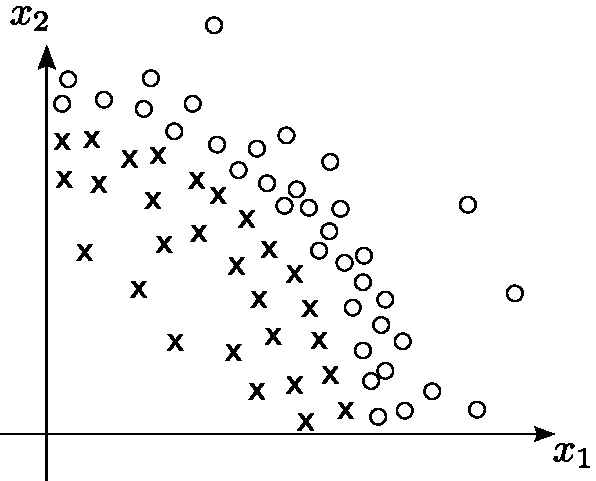
\includegraphics[width=0.4\textwidth]{img/circular}
     \mode<article>{
	\caption{A non-linearly separable classification problem.}
	}
	\label{fig:nonsepcirc} 
\end{figure}

\end{frame}

\begin{frame}\frametitle{\subsecname}

\question{Fit this parabola using only a connectionist neuron.}

\begin{figure}[ht]
     \centering
	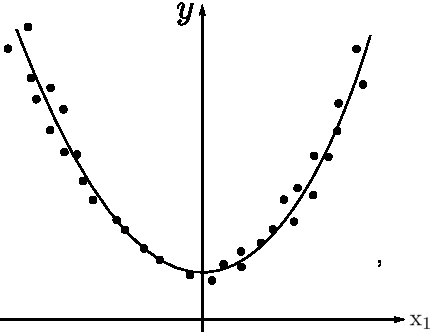
\includegraphics[width=0.4\textwidth]{img/section4_fig11_K2}
     \mode<article>{
	\caption{A non-linearly separable classification problem.}
	}
	\label{fig:nonsepcirc} 
\end{figure}

\question{How would you characterize any parabolic (quadratic) function?}

\pause
\slidesonly{\vspace{-5mm}}
\begin{equation}
y(x) = a x^{2} + b x + c =  w_{2} x^{2} + w_{1} x + w_{0}
\end{equation}

\end{frame}

\subsection{Nonlinear basis function}


\begin{frame}\frametitle{\subsecname}

Feature transformation $(\vec x\in \R^N)$:

\begin{equation}
\vec \phi: \vec x \mapsto \vec \phi(\vec x)
\end{equation}

\mode<article>{$\phi(\vec x)$ can transform our N-dim input $\vec x$ to another feature space of possibly higher dimensionality.
}
Expanding our feature space using \emph{Monomials} of highest degree $k$ (i.e. polynomial expansion):

\begin{align*}
\phi_i(\vec x) \in 
\{\;
&1, 
x_1\,,\, x_2, \ldots, x_N,
x_1^2\,,\, x_1 x_2, \ldots, x_1x_N,\ldots,\,x_N^2,\,\ldots\\
&x_1 x_N^{k-1}\,,\, x_1^k, \ldots, x_N^k
\}
\end{align*}

\begin{equation}
\phi_i(\vec x) \in \Big\{ \prod_{j=1}^N x_j^{a_j} \;\;: a_j \in \N_0 \;\; \text{with} \;\; 0 \, \le \, \sum_{j=1}^{N} a_j \le k  
\Big\} 
\end{equation}

where $i=1,\ldots d$.

Example: $k=9, N=2 \quad \Rightarrow \;\; d=55$


\end{frame}

\subsection{Preprocessing: Sphering}

\begin{frame}\frametitle{\subsecname}

Large $\lVert \vec x \rVert$ can lead to to very large $\phi_i(\vec x)$. \\

We want to decorrelate the transformed data and standardize it (keep variance of $\phi_i(\vec x)$ = 1)
\notesonly{
\emph{Sphering} is a preprocessing step that accomplishes both. 
The sphering transformation yields decorrelated input variables each with unit variance.
}
For every point $\alpha=1,\ldots,p$ from the training set:
\begin{equation}
\vec x^{(\alpha)}_\mathrm{sphered} = \vec \Lambda^{-\frac{1}{2}} \vec E^\top \vec x^{(\alpha)}_\mathrm{centered}.
\end{equation}

Here 
\begin{itemize}
 \item[]   
$\vec x^{(\alpha)}_\mathrm{centered} = \vec x^{(\alpha)} - \big<{\vec x}\big>\quad$ 
\notesonly{
denotes the centered data point $\alpha$ w.r.t. the center of the training data }
$\big<{\vec x}\big> = \frac{1}{p} \sum_{\alpha=1}^p \vec x^{(\alpha)}$,
\item[] $\vec E = (\vec e_1, \dots, \vec e_N)\quad$ is the eigenvector matrix and $\vec \Lambda = \mathrm{diag}(\lambda_1, \dots, \lambda_N)$ is the eigenvalue matrix for the eigendecomposition 
$$
\vec C \, \vec e_i = \lambda_i \vec e_i
$$ of the covariance matrix $\vec C$ with $C_{ij} = \frac{1}{p} \sum_{\alpha=1}^p x^{(\alpha)}_{\mathrm{centered},i} \, x^{(\alpha)}_{\mathrm{centered},j}$.
\end{itemize}


\end{frame}

\begin{frame}\frametitle{\subsecname}

Examining the properties of the data after sphering:

\begin{align}
\frac{1}{p}  \sum_{\alpha=1}^{p} \vec x^{(\alpha)}_\mathrm{sphered} &= \vec 0 \quad \text{(centered)},\\
\frac{1}{p}  \sum_{\alpha=1}^{p} (\vec x^{(\alpha)}_\mathrm{sphered})^{2} &=  1 \quad \text{(unit variance)},\\
\frac{1}{p}  \sum_{\alpha=1}^{p} x^{(\alpha)}_{\mathrm{sphered},i} \, x^{(\alpha)}_{\mathrm{sphered},j} &= 0 \quad \text{(zero covariance)},
\end{align}

\textbf{Important:} Reuse the same pre-processing (centering, sphering) on validation set. \notesonly{Do not recompute a separate mean or sphering transformation for the validation set.}
Also apply to test-set in case of a 3-way split.

\end{frame}

\subsection{Linear neuron for regression: Analytical solution}

\begin{frame}\frametitle{\subsecname}

\underline{Data}:\\

\begin{table}[h]
\begin{tabular}{rl}
transformed input & $\vec \phi^{(\alpha)} := \vec \phi(\vec x^{(\alpha)}) = \big (
\phi_{1}(\vec x^{(\alpha)}), \phi_{2}(\vec x^{(\alpha)}), \ldots, \phi_{d}(\vec x^{(\alpha)}) \big)^{\top}$ \\
label         & $y_{T}^{(\alpha)} \in \R$ \\
with & $\alpha = 1,\ldots,p$ and $\vec x$ has been centered and sphered.
\end{tabular}
\end{table}

\pause

\underline{Model}:\\[-5mm]

\notesonly{linear neuron on the \emph{the transformed} input:}
\begin{equation}
    y(\vec \phi; \vec w) = \vec w^{\top} \vec \phi = \sum_{i=1}^{d} w_{i} \phi_{i}(\vec x)\notesonly{\quad \text{(bias already incl.)}}
\end{equation}

quadratic cost function, L2 regularization. \pause Reuse solution for linear regression:

\begin{equation}
\vec w^{*} = \left( \vec \Phi \, \vec \Phi^{\top} + \lambda \vec I_{d}\right)^{-1} \vec \Phi \, \vec y_{\text{True}}^{\top}
\end{equation}

where $\vec \Phi = \left( \vec \phi^{(1)},\ldots, \vec \phi^{(\alpha)},\ldots, \vec \phi^{(p)}\right) \in \R^{d,p}$

\end{frame}

